\documentclass[10pt,a4paper]{article}

\setlength\topmargin{-48pt}
\setlength\headheight{0pt} 
\setlength\textwidth{7.0in} 
\setlength\textheight{9.5in}
\setlength\oddsidemargin{-30pt}
\setlength\evensidemargin{-30pt}
\setlength\parindent{0pt}

\usepackage{charter}

\frenchspacing

\usepackage{graphicx} 
\usepackage[ngerman]{babel}
\usepackage{amssymb,amsmath}
\usepackage{multicol}
\usepackage{url} 
\usepackage{enumitem}
\usepackage{marvosym}
\usepackage{wrapfig}
\usepackage[T1]{fontenc}
\usepackage{datetime}
\usepackage{url}
\newdateformat{mydate}{\monthname[\THEMONTH] \THEYEAR}
\usepackage[pdfpagemode=FullScreen, colorlinks=false]{hyperref} 
\usepackage{blindtext}
\usepackage{fancyhdr}
\pagestyle{fancy}

%-----------------------------------------------------------
% Kopf- und Fusszeile
\lfoot{\footnotesize
Mischa Knupfer \\
Andres Minder
}

\cfoot{Alle Infos auf:\\ \url{https://www.all-electronics.de/messung-der-relativen-luftfeuchtigkeit/}}
\rfoot{\footnotesize ~\\ Seite \thepage}

\renewcommand{\headrulewidth}{0.0pt}
\renewcommand{\footrulewidth}{0.4pt}
%-----------------------------------------------------------

%-----------------------------------------------------------
\newcommand{\HorRule}[1]{\noindent\rule{\linewidth}{#1}} 
\newcommand{\SepRule}{\noindent	
\begin{center}
\rule{250pt}{1pt} 
\end{center}
}
%-----------------------------------------------------------

%-----------------------------------------------------------
\newcommand{\NewsletterName}[1]{ % Newsletter title
\begin{center}
\Huge \usefont{T1}{fvs}{b}{n} % Use the Bera Sans Bold font
#1
\end{center}	
\par \normalsize \normalfont}

\newcommand{\JournalIssue}[1]{ % Date and issue number at the top of the newsletter
\hfill \textsc{04. Oktober 2018} % Right-aligned date and issue number
\par \normalsize \normalfont}

\newcommand{\NewsItem}[1]{ % News item title
\usefont{T1}{fvs}{n}{n} % Use the Bera Sans Normal font
\vspace{24pt}\large #1\vspace{3pt} % Print the title with space around it in a larger font size
\par \normalsize \normalfont}

\newcommand{\NewsAuthor}[1]{ % Author name under the item title
\hfill by \textsc{#1} \vspace{20pt} % Right-aligned author name in small caps with space after it
\par \normalfont}		

%----------------------------------------------------------------------------------------

%****************************************************************************************
\begin{document}

\JournalIssue{1} % Issue number

\NewsletterName{Luftfeuchtigkeitssensoren} % Newsletter title

\noindent\HorRule{3pt} \\[-0.75\baselineskip] % Thick horizontal rule
\HorRule{1pt} % Thin horizontal rule

%----------------------------------------------------------------------------------------

\vspace{0.5cm}
\SepRule
\vspace{-0.5cm}

\begin{center}
\begin{minipage}[h]{0.9\linewidth}
\begin{wrapfigure}{l}{0.42\textwidth}

\includegraphics[width=0.42\textwidth]{graphics/luftfeuchtigkeit.jpg}
\\
\end{wrapfigure}
	
\NewsItem{Grundlagen der Luftfeuchtigkeitsmessung}
\vspace{3pt}

%%======================================================================== Text Einfügen
\blindtext \\ \\
\blindtext \\ \\

\end{minipage}
\end{center}

\vspace{0.5cm}
\SepRule 
\vspace{0.5cm}

\NewsItem{Feuchtemessverfahren}

\begin{multicols}{2} 

%%======================================================================== Text Einfügen
{ \centering
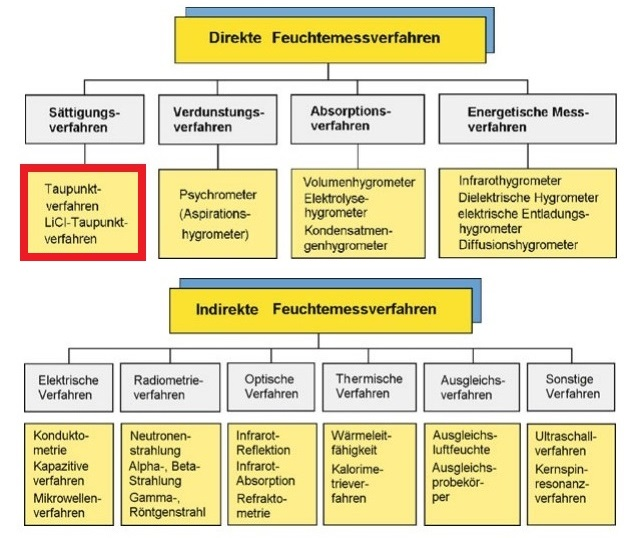
\includegraphics[width=\columnwidth]{graphics/verfahren.jpg}\\
\captionof{figure}{Direkte und indirekte Messverfahren \cite{Hesse2014}}
\label{dir_inddir_Messverf}
}
\vfill\columnbreak
Die Verfahren zur Feuchtemessung werden unterteilt in direkte und indirekte Methoden. Das direkte Feuchtemessverfahren trennt das Wasser direkt vom Feststoff. Das indirekte Verfahren misst Substanzeigenschaften, die durch den Wassergehalt messbar verändert werden, um danach über eine Kennlinie auf den Feuchtigkeitsgehalt zu schliessen. \cite{Hesse2014}\cite{Giessereilexikon}\\[0.5cm]
Die Luftfeuchtigkeit lässt sich mit verschiedenen Verfahren messen. MeteoSchweiz nutzt für die Temperatur- und Luftfeuchtemessung unter anderem das Instrument Thygan der Schweizer Firma Meteolabor AG, welches sehr genau und für extreme Witterungsbedingungen geeignet ist. Dieses Instrument nutzt das Verfahren mittels Taupunktspiegel, welches ein Sättigungsverfahren nutzt und somit zu den direkten Feuchtemessverfahren gehört. \cite{MeteoSchweiz2014}\\
\end{multicols}
\NewsItem{Elektronische Luftfeuchtigkeitsmessung}

\begin{multicols}{3}

%%======================================================================== Text Einfügen
\blindtext \\

\end{multicols} 

\begin{center}
\vspace{10pt}
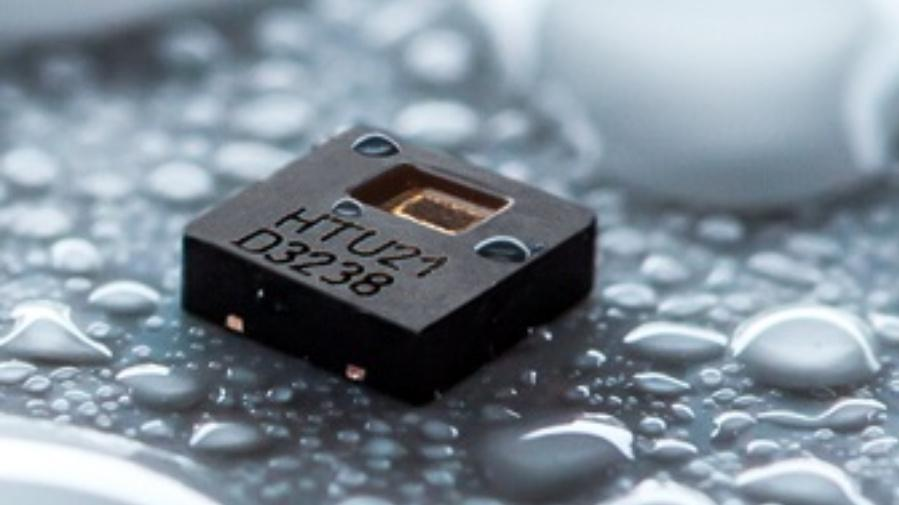
\includegraphics[width=0.8\linewidth]{graphics/placeholder.jpg} 
\par\large\textit{An interesting caption to this drab picture\ldots}
\vspace{10pt}
\end{center}

\end{document}
%****************************************************************************************